%----------------------------------------------------------------------------
\chapter{Background}
%----------------------------------------------------------------------------


%----------------------------------------------------------------------------
\section{Cloud Computing}
%----------------------------------------------------------------------------

\begin{itemize}
	\item \cite{AboveTheClouds}
	\begin{itemize}
		\item refers to both the applications delivered as services over the Internet and the hardware and systems software in the data centers that provide those services (these are often referred as software as a service) - here we focus on the applications
		\item cloud = data center hardware and software
		\item public cloud vs private cloud
		\item cloud pros - appearance of infinite computing resources, elasticity (to serve varying demand, or when demand is unknown), pay per use, transference of risk (of operation and of over/underprovisioning)
		\item 
	\end{itemize}
\end{itemize}

%----------------------------------------------------------------------------
\subsection{Software as a Service}
%----------------------------------------------------------------------------

\begin{itemize}
	\item https://en.wikipedia.org/wiki/Software\_as\_a\_service
	\begin{itemize}
		\item software delivery model (wikipedia)
		\item software is licensed on a subscription basis (wikipedia)
		\item software is centrally hosted (wikipedia)
	\end{itemize}
	\item \cite{AboveTheClouds}
	\begin{itemize}
		\item simplified software installation, maintainence, centralized control over versioning
		\item users can access the service anywhere, anytime, share and collaborate easily, keep data stored safely
		\item cloud computing allows deploying, scaling SaaS on demand
	\end{itemize}
	\item \cite{SaaSOppRisk}
	\begin{itemize}
		\item The SaaS model evolved from the application service provisioning (ASP) model, which emerged in the late 1990s as an on-demand software delivery option for (on-premise) commercial off-the-shelf application development. The ASP model involved vendor hosting, as well as managing and delivering application capabilities remotely from a data center accessed via the Internet. Technical issues that held ASP back during the 1990s included the initial design problems (i.e., few software applications were designed to be remotely accessible at that time), limited bandwidth availability, and slow Internet speeds. 
		\item multitenant architecture, there is only a single instance of the common code and data definitions of a given application on the vendor's server.
		\item the applications and infrastructure are shared across customers in the SaaS model
		\item SaaS model constrains clients' customization options of the software's main functionality and data structures
		\item it provides the vendor with more control over future development: 
	\end{itemize}
	
\end{itemize}


%----------------------------------------------------------------------------
\section{Microservices}
%----------------------------------------------------------------------------

before this, monolithic applications were popular

\begin{itemize}
	\item one deployment unit with many responsibilities
	\item tight coupling of different use-cases
	\item scalability issues
	\item vendor and technology lock in for the entire business application
\end{itemize}

----

\begin{itemize}
	\item \cite{MicroservicesMF}
	\begin{itemize}
		\item in short, the microservice architectural style is an approach to developing a single application as a suite of small services, each running in its own process and communicating with lightweight mechanisms, often an HTTP resource API. These services are built around business capabilities and independently deployable by fully automated deployment machinery. There is a bare minimum of centralized management of these services, which may be written in different programming languages and use different data storage technologies.
		
		Characteristics of a Microservice Architecture
		
		\item Componentization via Services
		\begin{itemize}
			\item here, a component is a unit of software that is independently replaceable and upgradeable.
			\item services are out-of-process (run in different processes, most likely on different machines - physical of virtual) components that communicate with mechanisms over the network
			\item services can be independently deployable (pros...)
			\item more explicit component interface
			\item Remote calls are more expensive than in-process calls, and thus remote APIs need to be coarser-grained, which is often more awkward to use (no free lunch)
		\end{itemize}
		\item Organized around Business Capabilities
		\item Smart endpoints and dumb pipes
		\begin{itemize}
			\item Applications built from microservices aim to be as decoupled and as cohesive as possible - they own their own domain logic and act more as filters in the classical Unix sense - receiving a request, applying logic as appropriate and producing a response.
			\item HTTP request-response, REST
			\item messaging over a lightweight message bus (RabbitMQ, Kafka)
		\end{itemize}
		\item Decentralized Governance
		\begin{itemize}
			\item no need to use the same technology stack for everything
			\item developers can use the right tools for each task and use-case
		\end{itemize}
		\item Decentralized Data Management
		\begin{itemize}
			\item each service maintains an own model of the world - its context is bounded so the component is only aware of the necessary information
			\item each component manages its own database, and databases can be accessed by other services only through their respective service - polyglot persistence
		\end{itemize}
	\end{itemize}
	\item \cite{ImplPatternsMicrosServices}
	\begin{itemize}
		\item Microservices is an application architectural style in which an application is composed of many discrete, network-connected components, termed microservices.
		\item the microservices approach stay focused on implementing clear business capabilities
		\item in the microservices architectural style, several smaller applications that each implement only part of the whole are built and packaged independently
		\item 5 simple rules drive the implementation of applications build using the microservices architecture
		\begin{itemize}
			\item Deploy applications as sets of small, independent services - one service per container
			\item Optimize services for a single function - this makes each service smaller and simpler to write and maintain (Rober Martin's "Single Responsibility Principle" \cite{RobertMartinOOP})
			\item Communicate via REST API and message brokers - limit options for simplicity, avoid tight coupling introduced by implicit communication through a database, ALL communication from service to service must be through the service API
			\item Apply Per-service CI/CD - it allows the different services to evolve at their own pace
			\item Apply Per-service HA/clustering decisions - The reality is that in a large system, not all services need to scale and can be deployed in a minimum number of servers to conserve resources. Others require scaling up to very large
			numbers.
		\end{itemize}
	\end{itemize}
	\item \cite{MicroservicesDocker}
	\begin{itemize}
		\item Microservices characteristics
		\begin{itemize}
			\item Small and focused - services should be modelled around specific business domain (not mimic organizational boundaries), each service should be treated as an independent application (own source code, CICD)
			\item Loosly coupled - Each microservice needs to be deployed as.needed without the necessary of coordination with other
			services’ owners
			\item Language-neutral - Microservices need to be built using technology that’s the developers are most comfortable with. The communication between the services is also language neutral, like HTTP or message brokers
			\item Bounded context - defines the details of a single domain (data model, domain model) and the integration points with other bounded contexts
		\end{itemize}
		\item Challenges in building a microservices architecture
		\begin{itemize}
			\item Failure Isolation - prefer quick failures, ability to determine where the failure happened
			\item Observability - health status, monitoring, logging - collect data and aggregate sensibly, helpful visualizations
			\item Automation requirement - as the number of services can grow rapidly
			\item High independence - 
			\item Testing - many moving parts, functional and non-functional aspects, distributed model
			\item Scaling - multiple instances, versions - many connections, service discovery mechanism, routing, configuration management issues
		\end{itemize}
	\end{itemize}
\end{itemize}


%----------------------------------------------------------------------------
\section{Dependability}
%----------------------------------------------------------------------------

Dependability of a computing system is the ability to provide service in which reliance can be justifiably placed \cite{DependabilityBMEMIT}. Meaning that based on conducting several analysis, evaluations and measurements it can be proofed that service satisfies the needs.

%----------------------------------------------------------------------------
\subsection{Attributes of Dependability}
%----------------------------------------------------------------------------

Dependability is a complex extra-functional characteristic of a system that consists of multiple attributes (based on the lectures in Systems Engineering \cite{DependabilityBMEMIT} and the Fundamental Concepts of Dependability \cite{FundamentalConceptsOfDependability}):

\paragraph{Availability} - Availability describes the probability of correct service in system. It also takes into account the time needed for repairs and maintenance tasks.

\paragraph{Reliability} - Reliability describes the probability of continuous correct service until the first failure. In case of mission critical systems, high reliability is an absolute requirement.

\paragraph{Safety} - A system is considered safe if it is free from unacceptable risk of harm. Harm can be defined in many different ways according to the domain in which the system operates.

\paragraph{Integrity} - Integrity assesses the absence of erroneous changes or alterations in the system. Integrity is a prerequisite for availability, reliability and safety as one cannot guarantee these attributes when there are misconfigurations in the system.

\paragraph{Maintainability} - Maintainability describes the possibility that the system is able to undergo repairs and improvements.


%----------------------------------------------------------------------------
\subsection{Dependability Metrics}
%----------------------------------------------------------------------------

The section above describing dependability presents well its compound nature, however, solely these definitions cannot be used to objectively assess the dependability of a given system in a deterministic way. Numerical representations of dependability -- so called dependability metrics -- are necessary in order to be able to conduct dependability analysis and measurements.

For sake of simplicity, one can use the notion that any given system has fundamentally two states, an Up and a Down state partitions. The Up partition stands for all the system states, where the system can provide correct service whereas the Down partitions denotes the states, where it cannot \cite{DependabilityBMEMIT}. It is important to mention, that providing correct service does not necessarily mean that the system is error free. Especially in case of highly distributed, dynamic environments, it is not feasible to guarantee the complete absence of errors for a long time. This leads to the fact that the essential question is not whether the system is error free, rather if it is able to function correctly and reliably.

The state of a system over time with respect to the before mentioned two state partitions can be visualized as shown is figure \ref{fig:system_state_partitions}. The function \(s(t)\) shows the system partition at any given time. During the intervals labeled with \(u_i\) the system was in the Up partition while during the intervals labeled with \(d_i\) the system was in the Down partition.


\begin{figure}[h]
	\centering
	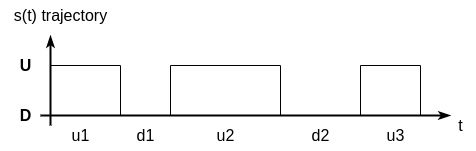
\includegraphics[width=100mm, keepaspectratio]{figures/system_state_partitions.png}
	\caption{ Partitioning the states of the system \cite{DependabilityBMEMIT} }
	\label{fig:system_state_partitions}
\end{figure}

%----------------------------------------------------------------------------
\subsubsection{Mean Values} \label{background-dep-metrics-mean-values}
%----------------------------------------------------------------------------

\paragraph{Mean Time to First Failure} - TODO

\begin{figure}[h]
	\centering
	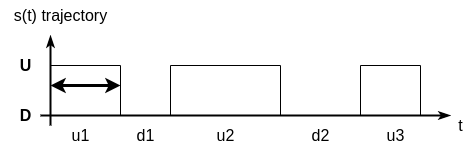
\includegraphics[width=100mm, keepaspectratio]{figures/MTFF.png}
	\caption{ Mean Time to First Failure \cite{DependabilityBMEMIT} }
	\label{fig:mtff}
\end{figure}

\paragraph{Mean Up Time} - TODO

\begin{figure}[h]
	\centering
	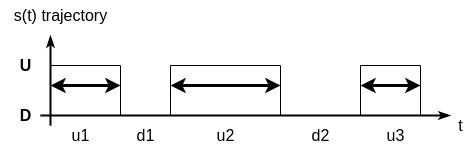
\includegraphics[width=100mm, keepaspectratio]{figures/MUT.png}
	\caption{ Mean Up Time \cite{DependabilityBMEMIT} }
	\label{fig:mut}
\end{figure}

\paragraph{Mean Down Time} - TODO

\begin{figure}[h]
	\centering
	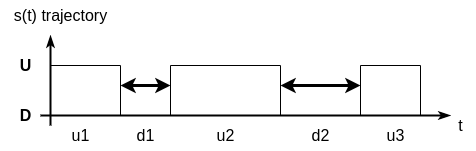
\includegraphics[width=100mm, keepaspectratio]{figures/MDT.png}
	\caption{ Mean Down Time \cite{DependabilityBMEMIT} }
	\label{fig:mdt}
\end{figure}

\paragraph{Mean Time Between Failures} - TODO

\begin{figure}[h]
	\centering
	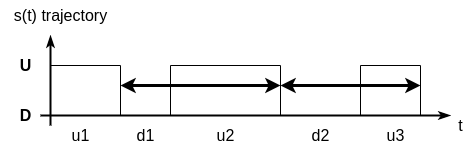
\includegraphics[width=100mm, keepaspectratio]{figures/MTBF.png}
	\caption{ Mean Time Between Failures \cite{DependabilityBMEMIT} }
	\label{fig:mtbf}
\end{figure}

%----------------------------------------------------------------------------
\subsubsection{Probability Functions} \label{background-dep-metrics-prob-funcs}
%----------------------------------------------------------------------------

\paragraph{Availability} - TODO

\[
a(t) = P\{ s(t) \in U \}
\]

\paragraph{Reliability} - TODO

\[
r(t) = P\{ s(t') \in U, \forall t' < t \}
\]


%----------------------------------------------------------------------------
\section{Kubernetes}
%----------------------------------------------------------------------------

%----------------------------------------------------------------------------
\subsection{Overview}
%----------------------------------------------------------------------------

%----------------------------------------------------------------------------
\subsection{Basic components}
%----------------------------------------------------------------------------

%----------------------------------------------------------------------------
\subsubsection{Namespace}
%----------------------------------------------------------------------------

%----------------------------------------------------------------------------
\subsubsection{Pod}
%----------------------------------------------------------------------------

+ assigning Pods to Nodes (PodAffinity)

%----------------------------------------------------------------------------
\subsubsection{ReplicaSet}
%----------------------------------------------------------------------------

%----------------------------------------------------------------------------
\subsubsection{Deployment}
%----------------------------------------------------------------------------

%----------------------------------------------------------------------------
\subsubsection{Service} \label{k8s-service}
%----------------------------------------------------------------------------

%----------------------------------------------------------------------------
\subsubsection{HPA}
%----------------------------------------------------------------------------

%----------------------------------------------------------------------------
\subsubsection{CRD}
%----------------------------------------------------------------------------

for Chaos Mesh experiments

%----------------------------------------------------------------------------
\subsection{Helm}
%----------------------------------------------------------------------------

%----------------------------------------------------------------------------
\subsection{AWS}
%----------------------------------------------------------------------------

%----------------------------------------------------------------------------
\subsubsection{CloudFormation}
%----------------------------------------------------------------------------

%----------------------------------------------------------------------------
\subsubsection{EKS}
%----------------------------------------------------------------------------


%----------------------------------------------------------------------------
\section{Metric collection - Monitoring}
%----------------------------------------------------------------------------

%----------------------------------------------------------------------------
\subsection{Time series}
%----------------------------------------------------------------------------

%----------------------------------------------------------------------------
\subsection{Prometheus}
%----------------------------------------------------------------------------

\begin{itemize}
	\item how it works
	\item the concept of exporters
\end{itemize}

%----------------------------------------------------------------------------
\subsubsection{PromQL} \label{background-promql}
%----------------------------------------------------------------------------

\begin{itemize}
	\item Introduce PromQL
	\item describe query functions that are later used to define dependability metrics
\end{itemize}

%----------------------------------------------------------------------------
\subsubsection{Prometheus Blackbox Exporter}
%----------------------------------------------------------------------------

%----------------------------------------------------------------------------
\subsubsection{Prometheus Adapter}
%----------------------------------------------------------------------------


%----------------------------------------------------------------------------
\subsection{Grafana}
%----------------------------------------------------------------------------


%----------------------------------------------------------------------------
\section{Chaos Engineering}
%----------------------------------------------------------------------------

\begin{itemize}
	\item 
\end{itemize}

%----------------------------------------------------------------------------
\subsection{Chaos Mesh} \label{background-chaos-mesh}
%----------------------------------------------------------------------------

%----------------------------------------------------------------------------
\subsubsection{Chaos Experiments}
%----------------------------------------------------------------------------

%----------------------------------------------------------------------------
\subsubsection{Scheduling Experiments}
%----------------------------------------------------------------------------



